\section{Identify the Deliveries}
In our project, we have to release four documents, moreover we have to do a code inspection of an existing well-­‐known open source project. So, we can naturally split our project in five deliveries:
\begin{itemize}
	\item RASD: Requirements Analysis and Specification Document
	\item DD: Design Document
	\item ITPD: Integrated Test Planning Document
	\item PP: Project Plan
	\item Code inspection and bug identification activity.
\end{itemize}
%FINAL PRESENTATION???

For each delivery, we have to respect a submission deadline, reported in the following table.
\begin{center}
  \begin{tabular}{ l | l }% p{10cm} }
   	\hline
	\textbf{DELIVERY} & \textbf{Submission deadline} 
   	\\ \hline
    RASD & 13/11/2016
    \\\hline
    DD & 11/12/2016
    \\\hline
    ITPD & 15/01/2017
    \\\hline
    PP & 22/01/2017
 	\\\hline
 	Code inspecion & 05/02/2017
   	\\\hline 
  \end{tabular}
\end{center}

Unfortunately, we can organize deliveries concurrently only in few cases. The RASD have to be completed before all the others, then the DD can be partially being done concurrently with the ITPD. The PP usually is done at the beginning of a project; in our case, it's done after the previous deliveries. The code inspection is executed on another project, so it can be done concurrently with every other delivery.

We decided to work on a delivery at a time in order to put all our efforts and reach the best possible result.

\newpage
\section{Scheduling}

In this chapter, we are going to provide the PowerEnJoy schedule. It takes account only of the main tasks that we have to complete for our specific project. Each task has also associated the name of the component of the team that released it, or both if we did the task together. 
\\The task during the project were split but here for a better understanding we reported only the main ones. We can also see that we frequently organized task concurrently.

\begin{center}
\begin{figure}[!ht]
  \centering
  \vspace{0.2cm}
  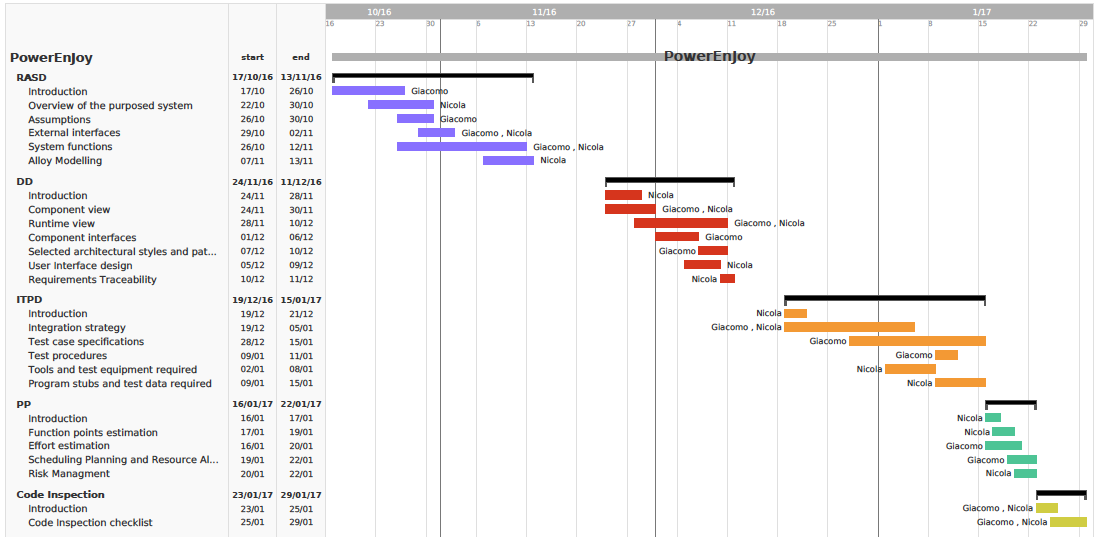
\includegraphics[width=1.3\textwidth]{/PP/PowerEnJoy_Gantt}\\
  \vspace{0.2cm}
  %\caption{Mockup for the login mobile page} 
  \label{fig:gantt} 
\end{figure}
\end{center}


